\chapter{Provedené experimenty}
V předchozí kapitole jsme se seznámili s algoritmy, které můžeme aplikovat i v našem prostředí.
V této kapitole se pomocí různých experimentů pokusíme nalézt agenty, kteří se budou chovat inteligentně.

Abychom ale mohli výsledky experimentů vyhodnocovat, případně je mezi sebou porovnávat, potřebuje mít na výsledky konkrétní kritéria.
Při testování obranného akčního plánu se ukázalo, že agent, který využívá pouze obranného akčního plánu k sestřelení nejbližšího asteroidu, se kterým vesmírné lodi hrozí srážka, dokázal díky dobré obraně zdatně přežívat ve hře mnoho kroků.
A zároveň je tento obranný agent kvůli využívání pouze jednoho akčního plánu dostatečně neinteligentní na to, abychom ho mohli použít jako referenčního agenta.

Jako kritérium pro hodnocení výsledků experimentů tedy bude sloužit souboj mezi výsledným agentem experimentu a obranným agentem.
A první, kterému se podaří zvítězit desetkrát, bude označen za vítěze. Výsledky těchto soubojů pak budou sloužit jako porovnání mezi jednotlivými výsledky provedených experimentů.

Druhým naším cílem bude nalézt agenty, kteří se budou chovat zajímavě ve smyslu pestrosti akcí a akčních plánů, nebo také zajímavě ve smyslu, že bude jejich chování působit jako chování lidského hráče.

\section{Genetické programování}
V prvních experimentech využijeme již zmíněného genetického programování. Nezbytným požadavkem je existence reprezentace jedince a fitness funkce, která mu přiřadí jeho hodnotu. 
Jedinec bude představovat rozhodovací funkci, která se na základě vstupních argumentů rozhodne, který akční plán bude vybrán.

V našem případě máme hru, kde spolu dva hráči soupeří a hra končí výhrou jednoho z hráčů.
Přesně tohoto můžeme ve fitness funkci jedince využít. 
Pokud chceme využít výsledku hry, jak jedinec ve hře dopadl, tak musíme nejprve zvolit proti jakému hráči bude jedinec, který je předmětem našeho zájmu, hrát.


Pro experimentování s genetickým programováním jsem zvolil knihovnu deap pro python. Zde lze jednoduše konfigurovat evoluční algoritmus na konkrétní řešený problém.
Stačí popsat jak reprezentovat jedince a jaká je jeho fitness funkce a zbytek knihovna vyřeší za nás.

\subsubsection{Reprezentace jedince}

Ve 3. kapitole jsme si vybudovali abstrakace v podobě senzorů a akčních plánů a těch zde budeme chtít využít.
Jedinec, podobně jako u symbolické regrese, je funkce, tedy může být reprezentován stromem.
Strom jedince budeme budovat prvkami z následující množiny terminálů a neterminálů.

\begin{itemize}
\item{
    Terminály:
    \begin{itemize}
        \item Vstupní argumenty rozhodovací funkce
        \item Celočíselné konstanty -1, 1, 3, 5, 10, 100
        \item Nulární funkce vracející výčtové hodnoty reprezentující zvolený akční plán  
    \end{itemize}    
    }    
\end{itemize}
Jako argumenty funkce jsem si zvolil následující hodnoty: délky všech čtyř akčních plánů a počet kroků před srážkou vesmírné lodi s asteroidem.
    Délky akčních plánů se pohybují v intervalu $(1,100)$, proto jsou číselné konstanty zvoleny tak, aby se jejich sčítáním a násobením lehce dosáhlo dalších hodnot z tohoto intervalu.


\begin{itemize}

\item{
    Neterminály:
    \begin{itemize}
        \item Aritmetické operace sčítání a násobení
        \item Funkce \emph{compare}
        \item Funkce \emph{if\_then\_else}
    \end{itemize}
}
\end{itemize}
Z aritmetický operací nám stačí sčítání a násobení. Operaci odčítání získáme pomocí sčítání a násobení konstantou -1. 
Hodnoty z intervalu $(1,100)$ jednoduše získáme také pomocí sčítání a násobení potřebných konstant, proto pro operaci dělení není důvod.
Všechny aritmetické operace jsou typu $([int,int], int)$.
Funkce \emph{compare} je typu $([int,int], Bool)$, vrací zda první argument je větší než druhý argument.
Poslední použitá funkce \emph{if\_then\_else} je typu 
\newline
$([Bool, ActionPlanEnum, ActionPlanEnum], ActionPlanEnum)$. 
Tato funkce dostává jako argumenty výraz typu bool a následně dvě hodnoty reprezentující akční plány. 
Na základě pravdivosti výrazu vrací funkce první nebo druhou z hodnot akčních plánů.

Tato popsaná reprezentace jedince bude použitá ve všech následujících experimentech. To, v čem se budou experimenty lišit, je způsob výpočtu fitness funkce a průběh evolučního algoritmu.

\newpage
\subsection{Experiment 1: Soupeření s obranným agentem}
Cílem tohoto experimentu bylo vyvinout agenta, který bude lepší než agent, který se řídí čistě obranným akčním plánem.
Výpočet fitness funkce proto zahrnuje zahrání 6 her současného jedince s obranným agentem a výsledek je průměr z hodnot každé z her.
Hra je pokaždé velmi náhodná, tedy zahrání jedné hry by mělo nízkou vypovídající hodnotu. Proto jsem pro přesnější informaci zvolil zahrání 6 her.
Hodnota zahrané hry se skládá z více částí.
\begin{itemize}
    \item Počet kroků trvání hry
        \newline
        Myšlenkou je zde, obzvláště v počátku evoluce, upřednostňovat takové jedince, kteří dokáží vydržet ve hře co nejdéle, tedy nejsou ve hře okamžitě poraženi.
        Pro představu, délky her se pohybují přibližně v intervalu $(900, 2900)$ kroků.
    \item Penalizace za nevyužití některého z plánů
        \newline
        Během hry se udržuje historie, kolikrát se agent rozhodl pro každý z akčních plánů.
        Za každý ze čtyř akčních plánů, který agent ani jednou během hry nezvolil bude přičtena penalizace -500. Cílem těchto penalizací je upřednostňovat takové jedince, kteří používají všechny akční plány a tím pádem mají pestřejší 
    \item Bonus (penalizace) za výhru (prohru)
        \newline
        Toto je asi nejdůležitější část. Pro zdůraznění rozdílu mezi vyhranými a prohranými hrami se v případě výhry přičtou k výsledku 2000 a v případě prohry se 2000 odečtou.
        Motivací mohou být následující dvě situace. Řekněme, že v jedné hře se podařilo jedinci dlouho bránit a dokázal vydržet 2500 kroků hry a poté prohrál. A v další situaci jedinec porazil soupeře v rychlých 1200 krocích. 
        Bez bonusu za vyhranou hru, by prohraná hra získala jedinci daleko vyšší hodnotu, než hra z druhé hry, kterou vyhrál.        
    
\end{itemize}

Algoritmus byl spuštěn s následujícími parametry:
\begin{itemize}
    \item Velikost populace: 30
    \item Pravděpodobnost křížení: 60\%
    \item Pravděpodobnost mutace: 20\%
    \item Počet generací: 100
    \item Metoda selekce: turnajová selekce
\end{itemize}

Výsledný nejlepší jedinec bohužel nesplnil naše očekávání a nedokázal obranného agenta porazit. 
V souboji jedinec nejen nedokázal konkurovat obrannému agentovi, ale ani se neřídí moc pestrou strategií.

V 95\% volil, stejně jako obranný agent, obranný akční plán a ve zbylých pár procentech volil všechny zbylé akční plány (viz \ref{Výsledek experimentu 01}).
Vyžívání všech akčních plánů bylo pravděpodobně dosaženo právě skrze vysokou penalizaci při nepoužití libovolného z nich, ale vidíme, že agent je volí spíš právě z tohoto důvodu, než že by je chtěl aktivně využívat v rámci své strategie.

\begin{figure}[p]\centering
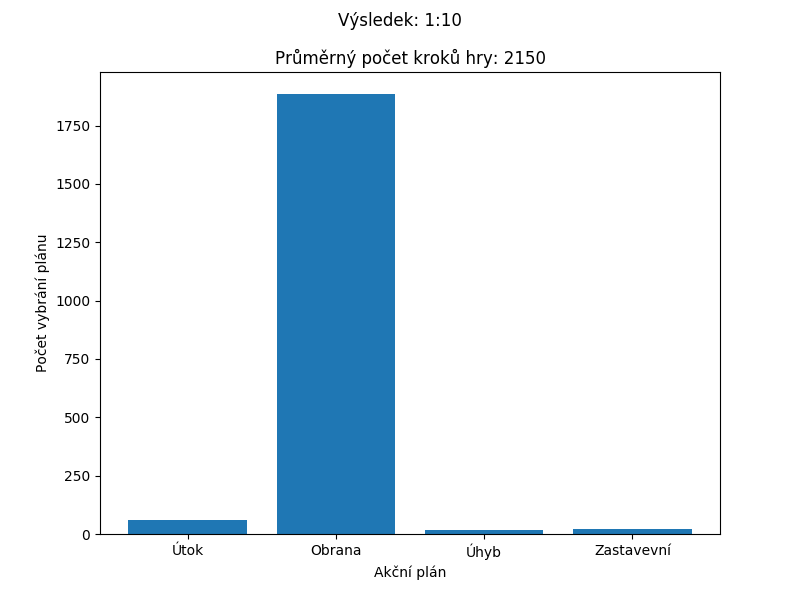
\includegraphics[width=125mm, height=100mm]{./Obrazky/Experiment01Results.png}
\caption{Výsledek experimentu 1}
\label{Výsledek experimentu 01}
\end{figure}



\newpage
\subsection{Experiment 2: Postupné zaměňování úspěšnějšího jedince}
V tomto experimentu nebylo cílem porazit konkrétního, stálého agenta jako v předchozím případě.
Cílem bylo postupně vybudovat nejzdatnějšího jedince.
Stejně jako v předchozím experimentu i zde fitness funkce spočívá v zahrání šesti her,
avšak zde nebudeme hrám přiřazovat žádnou číselnou hodnotu, ale spokojíme se s jednoduchou informací, který z agentů v dané hře zvítězil.
\par
Po celou dobu evoluce si budeme pamatovat současného nejlepšího jedince. 
Na začátku bude tento jedinec vybrán zcela náhodně.
Pak obvyklým způsobem vytvoříme populaci dalších jedinců a započneme evoluci.
Fitness funkce jedince bude počítat poměr, kolik ze šesti zahraných her jedinec vyhrál v souboji se současně nejlepším nalezeným jedincem.
Evoluce hledá řešení, která budou proti současnému nejlepšímu jedinci co nejúspěšnější.
V každé 3. generaci se následně kontroluje, zda již náhodou nebyl v populaci nalezen jedinec, který, pro danou situaci, nejlepšího jedince porazil alespoň v pěti ze šesti hrách.
Pokud ano, tak takový jedinec bude nově zvolen jako nejlepší a evoluce bude pokračovat stejným způsobem dál.
\par
Po výměně nejlepšího jedince musíme nově přepočítat fitness funkci všech stávajících jedinců v populaci, protože jejich současná hodnota se vztahovala k původnímu soupeři.
Rovněž musíme, ze stejného důvodu, smazat všechny jedince ze síně slávy (ang. Hall of fame), kde se průběžně ukládají nejlepší jedinci spolu s hodnotou jejich fitness funkce.

\par
Všechny tyto změny už nelze v knihovně deap nakonfigurovat přímočarým způsobem jako v předchozím experimentu, ale bylo zapotřebí upravit samotnou kostru evolučního algoritmu.

\par
Algoritmus byl spuštěn s následujícími parametry
\begin{itemize}
    \item Velikost populace: 10
    \item Pravděpodobnost křížení: 60\%
    \item Pravděpodobnost mutace: 20\%
    \item Počet generací: 450
    \item Metoda selekce: turnajová selekce
\end{itemize}

Nechali jsme výsledného agenta zahrát souboj s obranným agentem a tentokrát přinesl experiment daleko lepší výsledky.
Nalezený agent se oproti předchozímu experimentu dokázal naučit lépe utočit, volil útočný akční plán téměř ve 40\% případech a díky tomu dosáhl našeho primárního cíle. V Souboji porazil obranného agenta se skóre 10:0.
Nicméně ani tentokrát se agent nenaučil nic jiného než obranu a útok (viz \ref{Výsledek experimentu 02}). 

\newpage

 


\begin{figure}[p]\centering
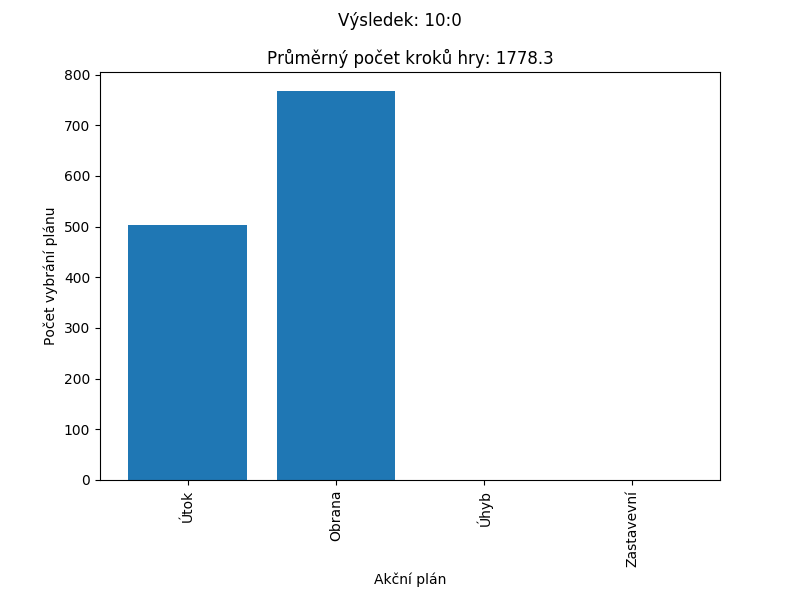
\includegraphics[width=125mm, height=100mm]{./Obrazky/Experiment02Results.png}
\caption{Výsledek experimentu 2}
\label{Výsledek experimentu 02}
\end{figure}




\newpage
\subsection{Experiment 3: Postupné zaměňování úspěšnějšího jedince bez obranného akčního plánu}

V předchozích experimentech se nám v obou případech podařilo vytvořit agenty, kteří v drtivé většině stavů rozhodují jen mezi obranným a útočným plánem.
To má za následek, že se agenti po celou dobu hry pouze otáčejí a střílejí, ale zůstavají při tom na jednom stejném místě.
V tomto experimentu tomuto problému zkusíme předejít, tím, že donutíme agenta bránit se uhýbáním namísto sestřelování nebezpečných asteroidů.

\par
Experiment bude probíhat stejným způsobem jako v předchozím případě, jen s tím rozdílem, že agentovi zakážeme používání obranného plánu. 
Z argumentů rozhodovací funkce odstraníme informaci o obranném plánu. 
A z množiny terminálů používaných při tvorbě programů odstraníme nulární funkci reprezentující obranný akční plán.

\par
To je vše co je potřeba změnit a zbylá logika může zůstat stejná jako v předešlém experimentu.

Algoritmus byl spuštěn s následujícími parametry
\begin{itemize}
    \item Velikost populace: 10
    \item Pravděpodobnost křížení: 60\%
    \item Pravděpodobnost mutace: 20\%
    \item Počet generací: 2000
    \item Metoda selekce: turnajová selekce
\end{itemize}

S výsledným agentem jsme opět provedli souboj s obranným agentem.
První čeho si můžeme všimnout je, že náš agent v souboji prohrál s výsledkem 2:10, tedy bez obranného akčního plánu nebyl schopný tak úspěšně konkurovat obrannému agentovi.
Druhá skutečnost, která stojí za povšimnutí je průměrná délka hry, ta byla v průměru přibližně o 500 kroků kratší než v předchozím experimentu. 
Z toho vyplývá, že využívání úhybného akčního plánu k přežívání není tak účinné, jako bránění se pomocí obranného akčního plánu. 
To ale není nijak překvapivé. Pro agenta je prostředí tím víc nebezepečné, čím více je v něm nebezpečných asteroidů. 
Používání úhybného akčního plánu vede k vyhnutí vesmírné lodi před nebezepčným asteroidem, né před jeho zníčením, jako je to u obranného akčního plánu. To má za následek, že v případě úhybného akčního plánu agent neredukuje počet nebezepčných asteroidů a mnohem dříve se dostane do stavu, kdy nemá šanci se roji asteroidů vyhnout. 

\par
Zajímavým výsledkem experimentu je také to, že, přestože agent používá, v rámci úhybného akčního plánu, akceleraci pro obranu velmi často, ani tentokrát nepoužívá zastavovací akční plán (viz \ref{Výsledek experimentu 03}).
To ukazuje, že zastavování letu není pro získání lepších výsledků stěžejní.
\par
Výsledný agent v souboji jednoznačně dosáhl špatných výsledků, ale pokud se na hru podíváme vizuálně, tak oproti agentům, kteří zůstávají po celou dobu hry na místě, působí agentovo chování z lidského pohledu mnohem zajímavěji.


\begin{figure}[p]\centering
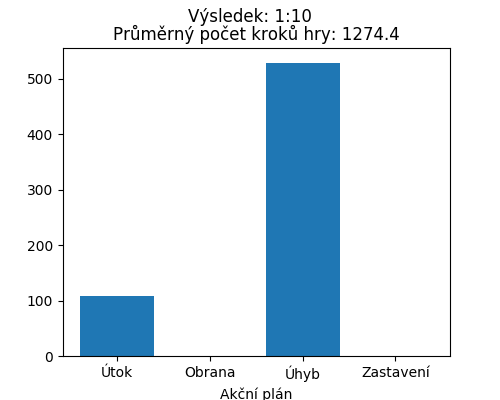
\includegraphics[width=125mm, height=100mm]{./Obrazky/Experiment03Results.png}
\caption{Výsledek experimentu 3}
\label{Výsledek experimentu 03}
\end{figure}





\section{Hluboké Q-učení}
Herní prostředí nám v každém kroku vrací odměnu, kterou oba z hráčů za jejich akci obdrželi. Tuto informaci jsme v experimentech provedených v rámci genetického programování, nevyužili, ale zde budou hrát velkou roli.
Za každý krok, kdy hra ještě neskončila získávají agenti automaticky odměnu 1. Na konci hry agent obdrží vysokou odměnu 2000 v případě výhry a v případě prohry naopak získá penalizaci v podobě odměny vysoké záporné hodnoty -1000.
Odměnu za výhru, nebo prohru získá agent až na úplném konci hry, to může ztěžovat učící proces. Proto prostředí dává agentům i průběžné menší odměny, pro lepší možnost učení se.

Konkrétně to jsou následující odměny:
\begin{itemize}
    \item Sestřelení asteroidu
        \newline
        Za každý sestřelený asteroid získává agent odměnu hodnoty 5.
    \item Zasažení asteroidem nepřátelské vesmírné lodi
        \newline
        Zranění nepřítele je právě to, co agent potřebuje pro přiblížění se vítězství, proto za každé takové zasažení získává od prostředí odměnu v hodnotě 20.
    \item Zasažení asteroidem vlastní vesmírné lodi
        \newline
        Takový stav je pro agenta znevýhodňující a cílem je se mu vyvarovat, proto za takovýto stav agent od prostředí dostává penalizaci v hodnotě -10.
\end{itemize}


\todo{presunout do kapitoly o deep q}
V rámci učení agentů budeme využívat epsilon-hladového (ang. epsilon-greedy) přístupu. V každém kroku q-učení volíme další akci a epsilon-hladový přístup nám v tom pomáhá následovně.
Vygenerujeme náhodnou hodnotou z intervalu $(0,1)$ a pokud je tato hodnota menší než hodnota epsilon, tak provedeme volbu akce náhodně, v opačném případě volíme nejlepší akce dle q-sítě.
Hodnota epsilon se na počátku inicializuje na hodnotu 1 a po každé zahrané hře se sníží vynásobením koeficientem menším než 1. 
Epsilon-hladový přístup způsobuje, že z počátku učení se zkoušejí náhodné akce a v průběhu přechází ze zkoušení nových akcí do prohledávání již osvědčených akcí.

\todo{presunout do kapitoly o deep q}
\par
Při trénování se nám stává, že měníme funkci, která odhaduje Q a tím je ovlivněno i chování agenta a odhady. K zachování větší stability trénování využijeme konceptu přehrávání zkušeností (ang. Experience replay).
Při hraní hry si v každém kroku ukládáme do paměti pětici současného stavu, provedené akce, obdržené odměny, stavu, do kterého jsme se dostali a informace zda hra neskončila.
Po konci zahrání hry následně náhodně vybíráme tyto pětice z paměti a trénování provádíme na nich.


\newpage
\subsection{Experiment 4: Soupeření s obranným agentem}
V 1. experimentu jsme za pomocí genetického programování hledali agenta, který je úspěšný v souboji s obranným jedincem. Pro určení jak agent v souboji obstál jsme využívali fitness funkci.
Zde, pomocí hlubokého q učení, budeme také učit agenta vzájemnými souboji s obranným agentem, ale budeme namísto fitness funkce používat pro trénování odměny.

S 1. experimentem zde bude také stejný přístup ke vstupům a výstupům. 
Na vstupu budou opět délky všech čtyř akčních plánů a počet kroků před srážkou vesmírné lodi s asteroidem.
A na výstupu čtyři hodnoty reprezentující výběr konkrétního akčního plánu.

Q učení spočívá v učení se rozhodování akcí. Akce zde v tomto pojetí však nebudou elementární akce, nýbrž akční plány. 
Q-síť bude tedy volit akční plány a proto zde budeme muset provádět mezikrok pro přechod od akčních plánů k akcím.
Nejprve vždy zvolíme akční plán a následně pro pokračování v simulaci hry z vybraného akčního plánu vybereme první akci.
V tomto experimentu budeme využívat přehrávání zkušeností, tj. budeme průběžně ukládat pětice informací o přechodech do dalších stavů. 
I Zde pro zapamatování si zkušenosti platí, že akcí budeme rozumět akční plán.


Parametry experimentu:
\begin{itemize}    
    \item Q-síť je hustá neuronová síť s pěti vstupy, čtyřmi výstupy a jednou skrytou vrstvou. 
    \item Během učení bude zahráno 1500 her.
    \item Konstanta pro snižování epsilon je nastavena na 0.998. To znamená, že například po zahrání 1400 her se bude v další hře volit akce náhodně jen v 6\% případů. 
\end{itemize}

\par
V souboji s obranným agentem se výslednému agentovi podařilo zvítězil pouze ve čtyřech hrách. 
Nepodařilo se nám tedy sice nalézt agenta, který by stabilně porážel obranného agenta, ale dosáhli jsme jiného zajímavého výsledku.
Velkým přínosem tohoto experimentu je pestrá strategie nalezeného agenta. Výsledný agent ve velkém zastoupení používá všechny akční plány (viz \ref{Výsledek experimentu 04}). 
Výsledkem je agent, který se brání nejen sestřelováním nepřátelských asteroidů, ale i vyhýbáním se. A díky tomu se agent také pohybuje a nezůstává jen staticky stát na stejném místě po celou dobu hry.
Toho se nám také podařilo dosáhnout ve 3. experimentu, ale ve srovnání s agentem získaným ze 3. experimentu je tento agent daleko více obranyschopný.




\begin{figure}[p]\centering
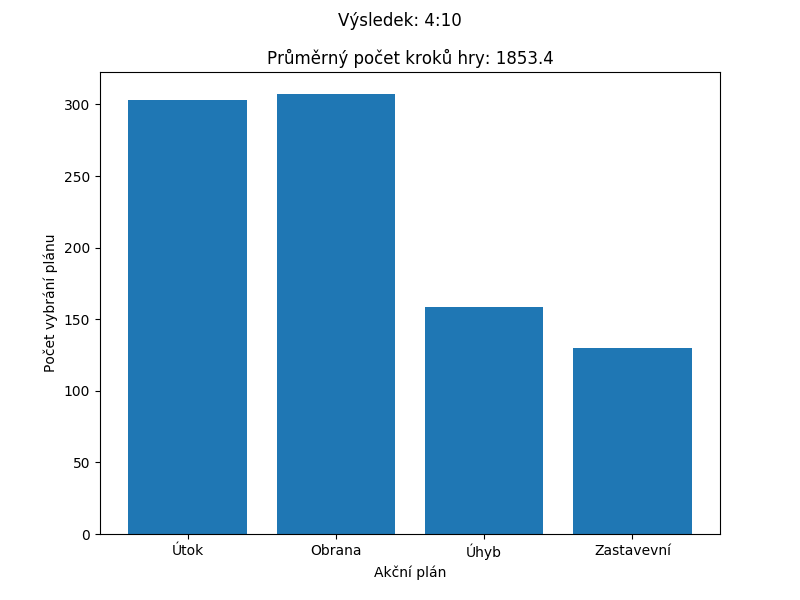
\includegraphics[width=145mm, height=110mm]{./Obrazky/Experiment04Results.png}
\caption{Výsledek experimentu 4}
\label{Výsledek experimentu 04}
\end{figure}


\newpage
\subsection{Experiment 5: Soupeření s obranným agentem - Rozšířeno}
V předchozím experimentu jsme dosáhli zajímavého chování agenta, ale nepodařilo se nám stabilně vyhrávat nad obranným agentem.
Zkusíme proto předchozí experiment rozšířit. 
V tomto experimentu zkusíme přidat další vstupní argumenty, které by mohli agentovi pomoct v rozhodování.

Přidané parametry:
\begin{itemize}
    \item Dvojice počtu zbývajících životů obou agentů            
    \item Počet nebezepčných asteroidů v blízké vzdálenosti od agenta
    \item Celkový současný počet nebezpečných asteroidů v celé hře
\end{itemize}
Snaha všech přidaných argumentů je rozšířit agentovi poznání o současném stavu hry a díky tomu dát agentovi možnost se komplexněji rozhodovat pro akční plány.

Parametry experimentu:
\begin{itemize}
    \item Q-síť je stejná síť jako v předchozím případě, jen namísto pěti vstupních argumentů, bude nyní přijímat vstupů devět.
    \item V tomto experimentu zkusíme kvůli rozšíření vstupních argumentů také prodloužit trénování sítě, proto bude v rámci trénování zahráno 3000 her.
    \item Adekvátně ke zvýšení počtu zahraných her také zvětšíme konstantu pro snižování epsilon z hodnoty 0.998 na 0.9989. Díky tomu bude stejné pravděpodobnosti 6\% pro volbu náhodné akce dosaženo přibližně po zahrání 2550 her.
\end{itemize}

\begin{figure}[p]\centering
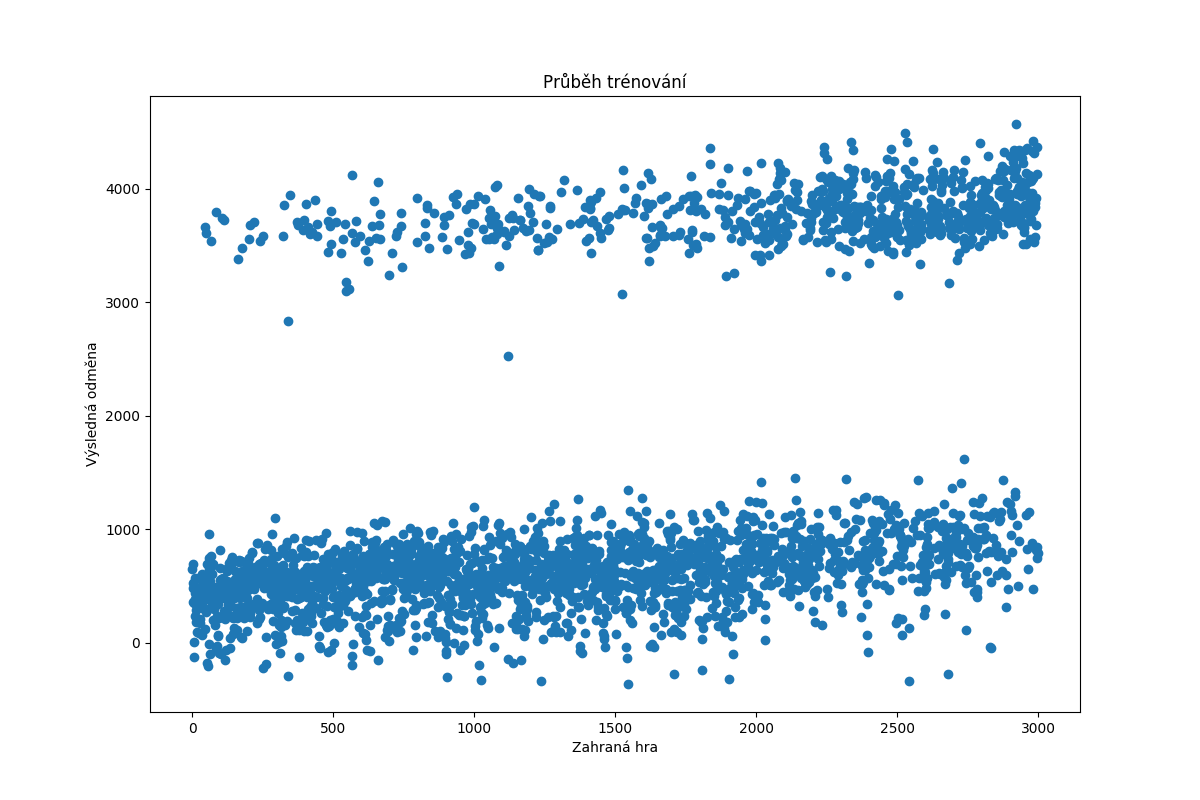
\includegraphics[width=145mm, height=110mm]{./Obrazky/Experiment05Training.png}
\caption{Průběh trénování v experimentu 5 - Výsledné odměny jsou součtem počtu kroků hry a odměny (resp. penalizace) za výhru (resp. prohru). Samotné tyto odměny tvoří rozdíl v hodnotě 3000, díky tomu je z obrázku zřetelné, ve kterých hrách agent vyhrál.}
\label{Průběh trénování experimentu 06}
\end{figure}




\begin{figure}[p]\centering
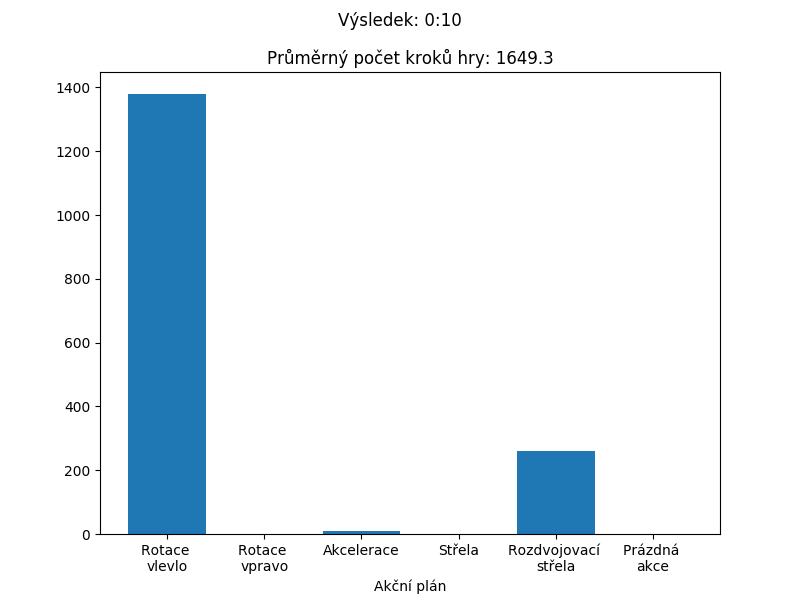
\includegraphics[width=145mm, height=110mm]{./Obrazky/Experiment05Results.png}
\caption{Výsledek experimentu 5}
\label{Průběh trénování experimentu 05}
\end{figure}


Výsledný agent dopadlo velmi úspěšně. Z průběhu trénování vidíme, že agent se velmi dobře učil a od přibližně 2300. hry (viz \ref{Průběh trénování experimentu 06}) už začal vyhrávat ve větší části her.
Rozšířením vstupních argumentů a přidání trénovacích her se nám podařilo zlepšit výsledek z předchozícho experimentu.
Agent sice ztratil pestrost akčních plánů, ale za to se významně zlepšil ve vyhrávání. Z výsledku 4:10 z předchozícho experimentu se zlepšil na 10:3.
Zajímavé na nalezeném agentovi je také jeho agresivita. Agent používá útočný akční plán přibližně dvakrát tak často jako obranný plán.

Při testování výsledného agenta jsem si všimnul, že zahrání jedné hry je časově značně náročné, přičemž to co při simulaci trvalo netriviální objem času bylo samotné dotazování q-sítě na akční plán.
Při snaze tento problém vyřešit jsem zjistil, že v některých stavech hry jsou všechny akční plány prázdné. 
Toto může nastat v případě kdy agent stojí na místě, není ohrožený žádným asteroidem a zároveň nenalezl žádný asteroid, kterým by mohl přímo ohrozit nepřítele.
V takovém stavu nemá velký smysl rozhodovat o volbě konkrétního akčního plánu. Proto jsem nastavil, že v takových případech agent rozhodování provádět nebude.

Podobně jsem také vypozoroval, že během jedné hry často nastane situaci, že právě jeden z akčních plánů je neprázdný. Překvapením pro mě bylo, že q-síť v některých takových případech volila jiný prázdný plán před tímto neprázdným.
Proto jsem nastavil vyjímku i pro tyto případy a v současnou chvíli platí, že když agent má k dispozici právě jeden neprázdný akční plán, tak ho volí automaticky bez dotazování se q-sítě.
Těmito opatřeními bylo dosaženo lepší časové náročnosti hraní hry a také byl agent v souboji úspěšnější. Zlepšení agenta si vysvětluji právě tím, že volba jakéhokoliv neprázdného plánu před prázdným je vždy výhodnější.


\todo{Naprogramovat spouštění experimentů}\newline
\todo{Popsat spouštění agentů}\newline





\newpage
\subsection{Experiment 6: Elementární agent proti obrannému agentovi}
V tomto experimentu zkusíme sestoupit od abstrakcí v podobě akčních plánů k elementárním akcím.
Tentokrát nebudeme q-síť používat k volbě akčního plánu, ale přímo k volbě elementární akce.
Výsledný agent bude volit vždy jen jednu akci, proto nebudeme moci využít koncept přepočítávání akčních plánů a agent se bude muset rozhodovat v každém kroku.
Opět budeme k trénování využívat soubojů s obranným agentem a učit se na základě odměn získaných od herního prostředí.

\par
K pěti elementárním akcím, pro které se bude agent rozhodovat, přidáme navíc také možnost prázdné akce. 
Nebudeme zde volit akční plány, proto tedy ani nemá dobrý smysl používat jejich délky jako argumenty pro rozhodování. Proto zde můžeme zvolit zcela jiný přístup.
Samotné simulace pro získání akčních plánů jsou výpočetně velmi náročné, a tedy díky tomu, že zde volíme jednodušší přístup, budeme schopni, oproti předchozím experimentům, zahrát v rámci trénování větší množství her.

\par
Jako vstupní argumenty jsem zvolil následující hodnoty:
\begin{itemize}
    \item Vektor současného pohybu vesmírné lodi
    \item Úhel natočení vesmírné lodi
    \item Počet uplynulých kroků od posledního výstřelu
    \item Relativní poloha nepřátelské lodi
    \item Relativní polohy tří nejbližších nebezpečných asteroidů
\end{itemize}

Parametry experimentu:
\begin{itemize}
    \item Q-síť je hustá neuronová síť s dvěmi skrytými vstvami, čtrnácti vstupními a šesti výstupními hodnotami.
    \item Díky nevyužívání akčních plánů bude hraní her rychlejší, proto pro trénování zahrajeme 10000 her.
    \item Konstanta pro snižoání epsilon je nastavena na hodnotu \todo{0.9998}
    \item V posledních 5\% her se nebude epsilon-hladový přístup používat a budou se volit nejlepší známé akce.
\end{itemize}


Výsledný agent proti obrannému agentovi nedopadl úspěšně. V souboji byl jednoznačně poražen se skóre 0:10.
A z přehledu používaných akcí během souboje můžeme i vypozorovat proč takto dopadl. Z elementárních operací se rozhodoval v drtivé většině pro rotaci vlevo a rozdvojovací střelu.
To v praxi znamená, že se agent naučil točit dokola a kdykoliv může, tak vystřelit. Tato strategie skutečně přináší nějaké výsledky.
Touto kombinací rotace a střelby se agent dokáže ubránit před srážkou s některými asteroidy, které by ho jinak zasáhly. Zároveň tímto způsobem sestřeluje netriviální množství asteroidů, které se kolem něho nacházejí a tím potenciálně staví nepřítele do ohrožení.
Avšak pro toto chování se agent rozhoduje bezmyšlenkovitě. 
Nemíří na žádné konkrétní asteroidy, ani na nepřátelskou loď.
Největší slabinou je, že agent se zde prakticky vůbec nenaučil bránit.
Veškeré asteroidy, před kterými se agent ubrání, zasáhne vesměs náhodně.


\begin{figure}[p]\centering
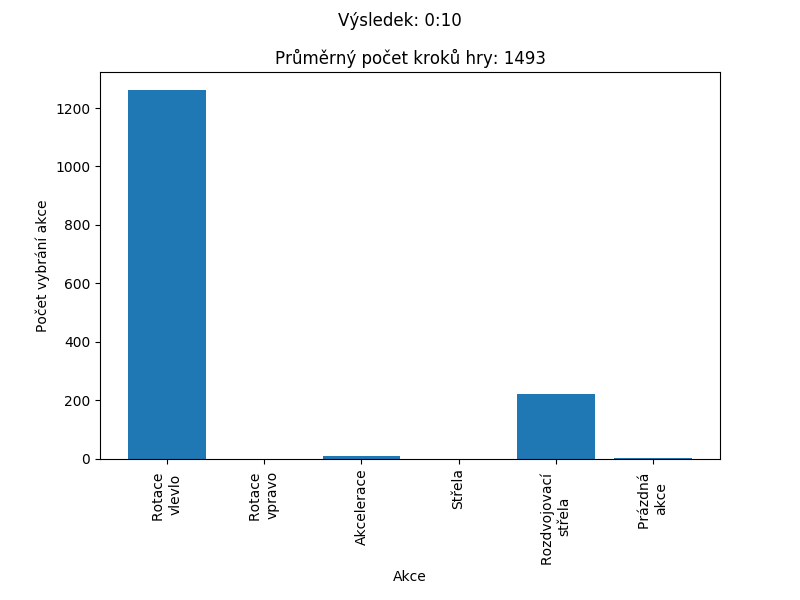
\includegraphics[width=145mm, height=110mm]{./Obrazky/Experiment06Results.png}
\caption{Výsledek experimentu 6}
\label{Výsledek experimentu 06}
\end{figure}
    



\newpage
\subsection{Experiment 7: Dva elementární agenti}
Tento experiment rozšiřuje experiment předchozí. Budeme opět pracovat s elementárním agentem reprezentovaným neuronovou sítí stejného formátu jako v předhozím případě.
Tentokrát ale nebudeme při trénování hrát hry proti obrannému agentovi, nýbrž proti dalšímu elementárnímu agentovi, který bude také zároveň trénován.
Budeme tedy provádět dvojí q-učení simultánně. Cílem je zde dosáhnout vzájemného adaptivního učení, kde se každý z agentů snaží zlepšovat proti svému nepříteli a postupně tak oba agenty zlepšovat.
\par


Parametry experimentu:
\begin{itemize}
    \item Každý agent bude reprezentován vlastní q-sítí stejného formátu jako v předchozím experimentu.
    \item Tím, že pro souboj nebudeme používat obranného agenta, ale dalšího elementárního agenta, ušetříme čas na výpočtu obranného agenta. V rámci trénování tedy zahrajeme 20000 her.  
    \item Konstanta pro snižoání epsilon je nastavena na hodnotu 0.9998
    \item V posledních 5\% her se nebude epsilon-hladový přístup používat a budou se volit nejlepší známé akce.
\end{itemize}


\begin{figure}[p]\centering
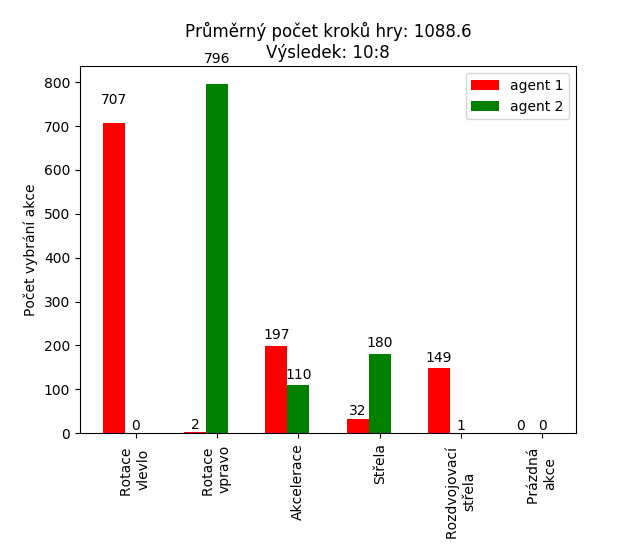
\includegraphics[width=145mm, height=110mm]{./Obrazky/Experiment07Results.png}
\caption{Výsledek experimentu 7}
\label{Výsledek experimentu 07}
\end{figure}


Výsledný souboj jsme výjmečně neprovedli proti obrannému agentovi, ale mezi vzniklými agenty mezi sebou.
Z přehledu souboje je vidět, že se agenti od předchozího experimentu nijak zásadně nezlepšili. Oba agenti se v drtivé většině stavů jen točí na jednu stranu.
Vidíme, že každý agent volí exklusivně pouze jednu stranu, na kterou se rotuje. 
Agent 1 se z přehledu souboje zdá být mírně pestřejší, kombinuje oba typy střel a navíc v téměř pětině stavů volil akceleraci.
Když jsem však vizuálně sledoval souboj agentů, tak žádný z agentů nejevil známky komplexnějšího chování. 